





% >>> j2l compat: xcolor / named-colour compatibility
\PassOptionsToPackage{dvipsnames}{color}
\PassOptionsToPackage{dvipsnames,svgnames,x11names,table}{xcolor}
\RequirePackage{xcolor}
\makeatletter\@namedef{ver@color.sty}{2021/01/01}\makeatother
\makeatletter\@ifundefined{providecolor}{}{%
  \providecolor{CarnationPink}{RGB}{128,128,128}
  \providecolor{Lavender}{RGB}{128,128,128}
  \providecolor{abstractcolor}{RGB}{128,128,128}
  \providecolor{rulecolor}{RGB}{128,128,128}
}\makeatother
% <<< j2l compat
\documentclass[10pt]{NSP1}

\IfFileExists{url.sty}{\usepackage{url}}{}
\IfFileExists{floatflt.sty}{\usepackage{floatflt}}{}

\IfFileExists{helvet.sty}{\usepackage{helvet}}{}
\IfFileExists{times.sty}{\usepackage{times}}{}

\IfFileExists{psfig.sty}{\usepackage{psfig}}{}
\IfFileExists{graphics.sty}{\usepackage{graphics}}{}

\IfFileExists{mathptmx.sty}{\usepackage{mathptmx}}{}
\IfFileExists{amsmath.sty}{\usepackage{amsmath}}{}
\IfFileExists{amssymb.sty}{\usepackage{amssymb}}{}
\IfFileExists{bm.sty}{\usepackage{bm}}{}

\IfFileExists{float.sty}{\usepackage{float}}{}

\IfFileExists{caption.sty}{\usepackage[bf,hypcap]{caption}}{}



\IfFileExists{xcolor.sty}{\usepackage[dvipsnames,table,xcdraw]{xcolor}}{}



\tolerance=1

\emergencystretch=\maxdimen

\hyphenpenalty=10000

\hbadness=10000



\topmargin=0.00cm



\def\sm{\smallskip}

\def\no{\noindent}



\def\firstpage{1}

\setcounter{page}{\firstpage}

\def\thevol{}

\def\thenumber{}

\def\theyear{}





\IfFileExists{graphicx.sty}{\usepackage{graphicx}}{}
\makeatletter
\def\biographyps#1#2{%
  \par\addvspace{21dd}\small\noindent
  \if!#1!\else
    \noindent\includegraphics[width=1in,height=1.25in,keepaspectratio]{#1}\par\smallskip
  \fi
  {\bfseries#2\unskip\ }\ignorespaces}
\def\endbiographyps{\par\addvspace{12pt}}
\makeatother
\IfFileExists{xcolor.sty}{\usepackage[table]{xcolor}}{}
\IfFileExists{array.sty}{\usepackage{array}}{}
\IfFileExists{cuted.sty}{\usepackage{cuted}}{\newenvironment{strip}{\par\medskip\noindent\begin{minipage}{\linewidth}}{\end{minipage}\par\medskip}}
\makeatletter
\newcommand\jltx@wideopen{\par\addvspace{\medskipamount}\noindent}
\newcommand\jltx@wideclose{\par\addvspace{\medskipamount}}
\newenvironment{jltxspan}
  {\if@twocolumn\let\jltx@spannext\strip\else\let\jltx@spannext\jltx@wideopen\fi\jltx@spannext}
  {\if@twocolumn\let\jltx@spanend\endstrip\else\let\jltx@spanend\jltx@wideclose\fi\jltx@spanend}
\makeatother
\newcommand\JLTXaboveplacement{\par\addvspace{6pt plus 2pt minus 2pt}\noindent}
\newcommand\JLTXbelowplacement{\par\addvspace{6pt plus 2pt minus 2pt}}
\widowpenalty=10000
\clubpenalty=10000

% >>> j2l compat: scalable Computer Modern (arbitrary font sizes)
\IfFileExists{type1cm.sty}{\usepackage{type1cm}}{}
\IfFileExists{fix-cm.sty}{\usepackage{fix-cm}}{}
% <<< j2l compat
\begin{document}
% >>> j2l compat: body-text size (+5%)
\makeatletter
\edef\JLTXbasesize{\f@size}
\@tempdimb=1.2\dimexpr\f@size pt\relax\edef\JLTXbaseskip{\strip@pt\@tempdimb}
\def\JLTXbodyscale{1.050}
\let\JLTX@normalsize\normalsize
\renewcommand\normalsize{%
  \JLTX@normalsize
  \@tempdima=\JLTXbodyscale\dimexpr\f@size pt\relax
  \@tempdimb=1.2\@tempdima
  \fontsize{\strip@pt\@tempdima}{\strip@pt\@tempdimb}\selectfont}%
\@ifundefined{@makecaption}{}{%
  \let\JLTX@makecaption\@makecaption
  \long\def\@makecaption#1#2{%
    \begingroup\fontsize{\JLTXbasesize}{\JLTXbaseskip}\selectfont
    \let\normalsize\JLTX@normalsize
    \JLTX@makecaption{#1}{#2}\endgroup}}%
\@ifundefined{thebibliography}{}{%
  \let\JLTX@thebibliography\thebibliography
  \def\thebibliography{%
    \fontsize{\JLTXbasesize}{\JLTXbaseskip}\selectfont\JLTX@thebibliography}}%
\makeatother
\normalsize
% <<< j2l compat

% >>> j2l: keep the journal banner with the title block
\makeatletter
\let\JLTXorig@newpage\newpage
\let\JLTXorig@clearpage\clearpage
\let\JLTXorig@cleardoublepage\cleardoublepage
\let\newpage\relax\let\clearpage\relax\let\cleardoublepage\relax
\makeatother
% <<< j2l




\titlefigurecaption{{\large \bf \rm Progress in Fractional Differentiation

and Applications}\\ {\it\small An International Journal}}



\title{A Fractional Fuzzy Dynamical Model for Math-Phobia with Optimal Learning Intervention Strategies}



\author{M. Ariyanatchi$^{1}$ \and P. Roselyn Besi2 I. Paulraj Jayasimman$^{1}$ \and Ali Akgül$^{2}$}

\institute{$^{1}$ Department of Mathematics, Academy of Maritime Education and Training (Deemed to be University), ECR, Kanathur, Chennai – 603 112, Tamil Nadu, India \\ $^{2}$ Siirt University, Art and Science Faculty, Department of Mathematics, 56100 Siirt, Türkiye}



\titlerunning{A Fractional Fuzzy Dynamical Model for Math-Phobia with Optimal Learning Intervention Strategies}

\authorrunning{M. Ariyanatchi et al.}





\mail{aliakgul@siirt.edu.tr}



\received{}

\revised{}

\accepted{}

\published{}



\abstracttext{This paper introduces a new six-compartment fuzzy fractional-order epidemic model that describes the spread and mitigation of math-phobia in student populations. The susceptible \(Ş(t)\), mathphobic \(M(t)\), not interested \(N(t)\), intervention-aware \(₳(t)\), interested \(ƚ(t)\), and recovered \(Ɍ(t)\) compartments capture key behavioural transitions influenced by psychological, social, and educational factors. Caputo-type fuzzy fractional differential equations are used to derive these dynamics, considering memory effects and epistemic uncertainty in the transmission and recovery rates. By applying fixed-point theory, we prove the existence and uniqueness of the solution under fuzzy initial conditions, hence guaranteeing mathematical coherence of the model.}



\keywords{Fuzzy fractional differential equations, Caputo derivative, Optimal control, Math-phobia Five-compartment model, Adomian decomposition, Fuzzy Laplace transform, educational intervention}



\maketitle
% >>> j2l: page breaking restored after the title block
\makeatletter
\let\newpage\JLTXorig@newpage
\let\clearpage\JLTXorig@clearpage
\let\cleardoublepage\JLTXorig@cleardoublepage
\makeatother
% <<< j2l





\par\medskip\noindent {\large\bfseries 1. Introduction\par}\smallskip

Mathematics anxiety, generally known as mathphobia, is a psychological condition in which one feels overwhelming fear, tension, and avoidance behaviours concerning mathematics. It has become so evident in people of all ages and levels of education; this has shorn away performance and confidence in individuals in mathematics-related tasks. Previous studies estimate that a strong percentage of students suffer from different mathphobia levels, which influences their academic and professional courses (Ashcraft \& Moore, 2009). Mathphobia is typically manifested by diminished problem-solving ability, negative attitude towards quantitative subjects, and increased cognitive interference associated with mathematical reasoning (Maloney \& Beilock, 2012; Hembree, 1990).

While mathphobia has not been identified as a clinical disorder, it does share characteristics with other anxiety disorders, such as avoidance behaviour, physiological stress responses, and impaired cognitive function associated with Dowker et al. (2016). Such attempts to understand and alleviate mathphobia have been made with the help of psychological testing, pedagogical interventions, and, increasingly in recent times, advanced mathematical modeling in order to describe its dynamic course.

Fuzzy fractional derivatives have developed as an influential tool to model complex, uncertain, and time-dependent phenomena like mathphobia. Fuzzy logic provides the facility for accommodating imprecise, ambiguous, and varied anxiety experienced by the individuals, which represents real-world behavioural uncertainty. Fractional calculus, with its memory effects and temporal dependence, enriches our understanding of the rrole that past experiences and interventions play in current math anxiety levels. Combination of fuzzy logic with fractional calculus therefore forms a comprehensive framework within which mathphobia dynamics can be analysed and specific intervention strategies can be designed.

A new fuzzy fractional derivative model for describing the progress of mathphobia is presented in this study, introducing optimal control methods to devise effective management approaches. This research develops the precision of modeling and mitigating the impact of mathphobia on learners by combining the nuanced representation capability of fuzzy fractional derivatives with the adaptability of optimal control.

\par\medskip\noindent {\large\bfseries Literature Review\par}\smallskip

Research on mathphobia has evolved from purely psychological and educational domains to include quantitative and computational modeling, thereby allowing for a much finer-grain understanding of dynamics of anxiety and the impact of interventions. In the foundational studies, the prevalence and cognitive effects of math anxiety were explored by Ashcraft \& Ridley (2005) and Hembree (1990), with early treatment approaches based on behavioral theories focused on desensitization and cognitive-behavioral therapy (Beilock \& Maloney, 2015; Dowker et al., 2016).

Fractional order mathematical models have been crucial for the correct representation of phenomena that involve memory and hereditary effects. This is because fractional derivatives explicitly represent the effects of previous states on the current behavior of a system, which is very crucial in chronic and recurrent psychological conditions like mathphobia. This provides higher fidelity in modeling compared to traditional integer-order models (Maayah \& Arqub, 2023; Kongson et al., 2021). Such models have carved success through epidemiology and psychology by capturing persistence, relapse, and gradual recovery phases.

Along with this, in the context of psychological measurements, fuzzy mathematical models address uncertainty and imprecision by treating each variable as a fuzzy set with degrees of membership rather than precise values. Such methodology goes side by side with the nature of mathphobia because in reality it has a spectrum-like manifestation across individuals and contexts (Liang et al., 2021; Van Hoa, 2019). Integrating such frameworks into FFDEs may establish a powerful tool to model nonlinear, uncertain, and history-dependent processes related to psychological and educational systems (Arshad, 2024; Qayyum et al., 2024).

Recent analyses have employed compartmental and structural equation models to characterize the different stages of psychological anxiety and some possible mitigation pathways (Abi et al., 2023; Mitropoulou et al., 2022; Sheinov \& Dziavitsyn, 2021). Other works, such as Juhari et al. (2024) and Alemneh \& Alemu (2021), illustrate the use of optimal control theory combined with fractional models in the optimization of intervention timing, intensity, and resources for higher efficacy and cost-effectiveness. Sheinov \& Dziavitsyn (2021) present the development of a fractional behavioral model that involves cognitive, emotional, and social factors of addiction, offering insights transferable to mathphobia dynamics.

In this respect, the fuzzy fractional Caputo derivative provides a privileged mathematical framework in developing models of real systems that are driven by incomplete or imprecise information with a dependency on the history. The nonlinearities, imprecision, and noise in data can be better understood and addressed using the fuzzy fractional Caputo model compared to its classical/integer-order counterparts in behavioral studies (Liang et al., 2021; Van Hoa, 2019).

Complementary to these models, optimal control theory provides the decision-making frameworks needed to optimize the timing of interventions, their intensities, and resource allocation. Such works have been developed by Juhari et al. (2024), Alemneh \& Alemu (2021). Combined fuzzy fractional and optimal control-based models represent state-of-the-art tools to devise adaptive, data-driven policies toward the reduction of mathphobia.

Whereas there has been some progress with regard to fractional modeling in psychology and education, applications to mathphobia specifically remain limited, but promising. This study tries to fill the gap by presenting a fuzzy fractional mathematical model with optimal control for enhanced analysis and better management of mathphobia.

\par\medskip\noindent {\large\bfseries Novelty and Objectives\par}\smallskip

In this paper, a new fuzzy fractional derivative model for mathphobia is presented, utilizing the Caputo fractional operator and fuzzy logic to enhance the descriptive accuracy regarding the development of anxiety over time. An optimal control approach is integrated into the model in order to identify strategies of intervention that are both effective and adaptive, which alter trajectories of anxiety. This two-pronged approach goes much further toward understanding the dynamics underlying mathphobia by incorporating behavioral uncertainty, long-term dependencies, and real-time control measures-a comprehensive methodology hardly explored so far in the literature.

The organization is as follows: The second section gives some necessary mathematical preliminaries, including fuzzy sets, fractional calculus, and the Atangana–Baleanu–Caputo fractional derivative. In the third section, the paper develops the fuzzy fractional model relevant to mathphobia, outlining the methods of incorporating fuzzy operators and parameters that might describe anxiety dynamics. Section four discusses the mathematical analysis, focusing on stability and the existence of solutions of the proposed model. Section five describes the numerical approaches used, with an emphasis on the use of fuzzy fractional Laplace transforms for solving and simulating the system. Numerical results are presented in section six, where an interpretation of these results is made within the context of intervention strategies and how they might best be used to manage math anxiety. Finally, the seventh section concludes the paper, summarizing key findings and suggesting avenues for future research. This structure allows a comprehensive investigation into the topic, starting from theoretical foundations to practical implications.

\par\medskip\noindent {\large\bfseries 2. Model Construction\par}\smallskip

The proposed fuzzy fractional Caputo model divides the student population into six compartments: susceptible \(Ş(t)\), mathphobic \(M(t)\), not interested \(N(t)\), intervention-aware \(₳(t)\), interested \(ƚ(t)\), and recovered \(Ɍ(t)\). New students enter the system at rate \(\Lambda\). Susceptible students can develop mathphobia due to academic stress or peer influence at rate \(\beta_{1}\), or become disinterested at rate \(\beta_{2}\). Positive educational exposure enables susceptible students to become interested at rate \(\theta\). Mathphobic students might reduce anxiety and transition to the not interested group at rate \(\alpha\) or enter the intervention-aware category if they join anxiety reduction programs, at rate \(\delta_{1}\). Similarly, not interested students can move into intervention-aware at rate \(\delta_{2}\). Recoveries from mathphobia, disinterest, interest, and intervention groups occur at rates \(\gamma_{1},\gamma_{2},\gamma_{3},\) and \(\gamma_{4}\), respectively. The natural dropout rate \(\mu\) affects all compartments. These dynamics are captured using the fuzzy fractional Caputo derivative operator of order \(\vartheta\), denoted here as \(0FFCD_{t}^{\vartheta}\).

The system of fuzzy fractional differential equations is given by:

\(0FFCD_{t}^{\vartheta}\ Ş = \widetilde{\Lambda} - \widetilde{\beta_{1}}\ ŞM - \widetilde{\beta_{2}}\ ŞN - \left( \ \widetilde{Ө} + \widetilde{\mu\ } \right)Ş\)

\(0FFCD_{t}^{\vartheta}\ M\ = \widetilde{\beta_{1}}\ ŞM - \left( \widetilde{\Upsilon_{1}} + \ \widetilde{\alpha} + \widetilde{\delta_{1}} + \widetilde{\mu\ } \right)M\)

\(0FFCD_{t}^{\vartheta}N = \widetilde{\beta_{2}}\ ŞN + \widetilde{\alpha}M - \left( \widetilde{\Upsilon_{2}} + \widetilde{\delta_{2}} + \widetilde{\mu\ } \right)N\)

\(0FFCD_{t}^{\vartheta}\ ₳ = \widetilde{\delta_{1}}M + \widetilde{\delta_{2}}N - \left( \widetilde{\Upsilon_{3}} + \widetilde{\mu\ } \right)₳\)

\(0FFCD_{t}^{\vartheta}ƚ = \widetilde{Ө}Ş - \left( \widetilde{\Upsilon_{4}} + \widetilde{\mu\ } \right)ƚ\)

\(0FFCD_{t}^{\vartheta}\ Ɍ = \widetilde{\Upsilon_{1}}M + \widetilde{\Upsilon_{2}}N + \widetilde{\Upsilon_{3}}₳ + \widetilde{\Upsilon_{4}}ƚ - \widetilde{\mu\ }Ɍ\)

The initial conditions for the model are defined as:

\[
Ş(0) = Ş_{0},M(0) = M_{0},N(0) = N_{0},₳(0) = ₳_{0},ƚ(0) = ƚ_{0},Ɍ(0) = Ɍ_{0},
\]

where these values represent the initial state of students in each compartment at time zero.

\par\medskip\noindent {\large\bfseries Table 1: Parameter Description Table\par}\smallskip

\JLTXaboveplacement \begin{jltxspan}%
\noindent\begin{minipage}{\linewidth}%
\centering
{\small
\begin{tabular}{|>{\centering\arraybackslash}p{\dimexpr 0.1478\linewidth-2\tabcolsep-\arrayrulewidth\relax}|>{\raggedright\arraybackslash}p{\dimexpr 0.8411\linewidth-2\tabcolsep-\arrayrulewidth\relax}|}
\hline
\cellcolor[HTML]{F2F2F2}\textbf{Parameter} & \cellcolor[HTML]{F2F2F2}\textbf{Description} \\
\hline
Λ & Recruitment rate of new students entering the system \\
\hline
\[\beta_{1}\] & Rate at which susceptible students develop mathphobia \\
\hline
\[\beta_{2}\] & Rate at which susceptible students become not interested \\
\hline
\[\theta\] & Rate of susceptible students gaining interest via positive exposure \\
\hline
\[\alpha\] & Rate at which mathphobic students become not interested \\
\hline
\[\delta_{1}\] & Rate at which mathphobic students join intervention programs \\
\hline
\[\delta_{1}\] & Rate at which not interested students join intervention programs \\
\hline
\[\gamma_{1}\] & Recovery rate from mathphobia to recovered \\
\hline
\[\gamma_{2}\] & Recovery rate from not interested to recovered \\
\hline
\[\gamma_{3}\] & Recovery rate from interested to recovered \\
\hline
\[\gamma_{4}\] & Recovery rate from intervention-aware to recovered \\
\hline
\[\mu\] & Natural dropout rate (graduation, transfer, etc.) \\
\hline
\[\vartheta\] & Order of fuzzy fractional Caputo derivative \\
\hline
\end{tabular}}
\captionof{table}{Table}%
\end{minipage}%
\end{jltxspan}\JLTXbelowplacement 

\par\medskip\noindent {\large\bfseries 3.Mathematical analysis of model\par}\smallskip

\par\medskip\noindent {\large 3.1. Positivity and boundedness of the crisp model\par}\smallskip

The positivity and boundedness of the proposed model are crucial aspects for which theorems, along with proofs, are provided as follows:

Theorem 1. The solution trajectories of the crisp model (1) are all positive at any time instant in \({\ R}_{+}^{6}\).

Proof. From the system (4), we get

\({0FFCD_{t}^{\vartheta}\ Ş(t)|}_{Ş = 0} = \Lambda\\), \({0FFCD_{t}^{\vartheta}\ M(t)|}_{ƚ = 0} = 0\), \({0FFCD_{t}^{\vartheta}\ N(t)|}_{ƚ = 0} = \widetilde{\alpha}M,\\)

\({0FFCD_{t}^{\vartheta}\ ₳(t)|}_{₳ = 0} = \widetilde{\delta_{1}}M + \widetilde{\delta_{2}}N\), \({0FFCD_{t}^{\vartheta}\ ƚ(t)|}_{ƚ = 0} = \widetilde{Ө}Ş\), \({0FFCD_{t}^{\vartheta}\ Ɍ(t)|}_{Ɍ = 0} = \widetilde{\Upsilon_{1}}M + \widetilde{\Upsilon_{2}}N + \widetilde{\Upsilon_{3}}₳ + \widetilde{\Upsilon_{4}}ƚ\).

All the above-mentioned rates are nonnegative, and so are the solution trajectories in the non-negative of \({\ R}_{+}^{6}\).

Theorem 2. The solution of crisp \(ŞMN₳\ ƚɌ\) model (1) is uniformly bounded.

Proof.

Let (𝑡) = \(Ş(t)\) + \(M\) (𝑡) + \(N\)(𝑡) +\(₳\\)(𝑡) + \(ƚ\)(𝑡) + \(Ɍ\)(𝑡), then we obtain

\(0FFCD_{t}^{\vartheta}N(t) +\)𝜇𝑁 = \(\Lambda\)

Integrating both sides of above equation and using initial conditions for infections outbreak we get

\[
e^{\mu t}N = \frac{\Lambda e^{\mu t}}{\mu}\ + \ \left( N_{0} - \frac{\ \Lambda}{\mu} \right)
\]

\[
N = \frac{\Lambda}{\mu}\ + \ \left( N_{0} - \frac{\ \Lambda}{\mu} \right)e^{- \mu t}
\]

as \(t \rightarrow \infty\), we obtain

\(Ş(t)\ + \ M\ (t)\ + \ N(t)\ + ₳\ (t)\ + \ ƚ(t)\ + \ Ɍ(t) \leq \ \frac{\Lambda}{\mu}\)

\[
N(t) \leq \ \frac{\Lambda}{\mu}
\]

\[
0 \leq N(t)\ \leq \ \frac{\Lambda}{\mu}
\]

Hence, all the solution trajectories of system (1) are bounded in the spanned output space.

\par\medskip\noindent {\large 3.2. Existence and Uniqueness Results\par}\smallskip

This section describes the existence and distinctiveness of the solution to the following fuzzy fractional model. Here, this study looked into a set of fuzzy fractional-order differential equations in the sense of Atangan-Baleanu Caputo, which depicts an epidemic model of childhood sickness with initial data uncertainty. For \(0 < \vartheta \leq 1\),

\(\{ 0FFCD_{t}^{\vartheta}\ Ş(t) = \widetilde{\Lambda} - \widetilde{\beta_{1}}\ ŞM - \widetilde{\beta_{2}}\ Ş\ N - \left( \ \widetilde{Ө} + \widetilde{\mu\ } \right)Ş\ \ \ \ 0FFCD_{t}^{\vartheta}\ M(t) = \widetilde{\beta_{1}}\ ŞM - \left( \widetilde{\Upsilon_{1}} + \ \widetilde{\alpha} + \widetilde{\delta_{1}} + \widetilde{\mu\ } \right)M\ \ 0FFCD_{t}^{\vartheta}\ N(t) = \widetilde{\beta_{2}}\ ŞN + \widetilde{\alpha}M - \left( \widetilde{\Upsilon_{2}} + \widetilde{\delta_{2}} + \widetilde{\mu\ } \right)N\ \ 0FFCD_{t}^{\vartheta}\ ₳(t) = \widetilde{\delta_{1}}M + \widetilde{\delta_{2}}N - \left( \widetilde{\Upsilon_{3}} + \widetilde{\mu\ } \right)₳\ 0FFCD_{t}^{\vartheta}\ ƚ(t) = \widetilde{Ө}Ş - \left( \widetilde{\Upsilon_{4}} + \widetilde{\mu\ } \right)ƚ\ \ 0FFCD_{t}^{\vartheta}\ Ɍ(t) = \widetilde{\Upsilon_{1}}M + \widetilde{\Upsilon_{2}}N + \widetilde{\Upsilon_{3}}₳ + \widetilde{\Upsilon_{4}}ƚ - \widetilde{\mu\ }Ɍ\ \ \\) (2)

Now the right-hand side of (2) becomes,

\(\{\psi_{1}\left( t,Ş(t) \right) = \widetilde{\Lambda} - \widetilde{\beta_{1}}\ ŞM - \widetilde{\beta_{2}}\ Ş\ N - \left( \ \widetilde{Ө} + \widetilde{\mu\ } \right)Ş\ \ \ \ \ \psi_{2}\left( t,M(t) \right) = \widetilde{\beta_{1}}\ ŞM - \left( \widetilde{\Upsilon_{1}} + \ \widetilde{\alpha} + \widetilde{\delta_{1}} + \widetilde{\mu\ } \right)M\ \ \psi_{3}\left( t,N(t) \right) = \widetilde{\beta_{2}}\ ŞN + \widetilde{\alpha}M - \left( \widetilde{\Upsilon_{2}} + \widetilde{\delta_{2}} + \widetilde{\mu\ } \right)N\ \psi_{3}\left( t,₳(t) \right) = \widetilde{\delta_{1}}M + \widetilde{\delta_{2}}N - \left( \widetilde{\Upsilon_{3}} + \widetilde{\mu\ } \right)₳\ \psi_{4}\left( t,ƚ(t) \right) = \widetilde{Ө}Ş - \left( \widetilde{\Upsilon_{4}} + \widetilde{\mu\ } \right)ƚ\ \ \psi_{5}\left( t,Ɍ(t) \right) = \widetilde{\Upsilon_{1}}M + \widetilde{\Upsilon_{2}}N + \widetilde{\Upsilon_{3}}₳ + \widetilde{\Upsilon_{4}}ƚ - \widetilde{\mu\ }Ɍ\ \ \\) (3)

Where the fuzzy functions are \(\psi_{1},\psi_{2},\psi_{3},\psi_{4},\psi_{5}\), \(\psi_{6}\) then, for \(ɤ \in \lbrack 0,1\rbrack\), model (2) gets the form

\(\{ 0FFCD_{t}^{\vartheta}\ Ş(t) = \psi_{1}\left( t,Ş(t) \right)\ 0FFCD_{t}^{\vartheta}\ M(t) = \psi_{2}\left( t,M(t) \right)\ 0FFCD_{t}^{\vartheta}\ N(t) = \psi_{3}\left( t,N(t) \right)\ 0FFCD_{t}^{\vartheta}\ ₳(t) = \psi_{4}\left( t,\ ₳(t) \right)\ 0FFCD_{t}^{\vartheta}\ ƚ(t) = \psi_{4}\left( t,\ ƚ(t) \right)\ 0FFCD_{t}^{\vartheta}\ Ɍ(t) = \psi_{5}\left( t,Ɍ(t) \right)\\) (4)

With fuzzy initial conditions

\(\widetilde{Ş}(0,ɤ) = \left\lbrack \underline{Ş}(0,ɤ),\underline{Ş}(0,ɤ) \right\rbrack\)

\(\widetilde{M}(0,ɤ) = \left\lbrack \underline{M}(0,ɤ),\underline{M}(0,ɤ) \right\rbrack\)

\(\widetilde{N}(0,ɤ) = \left\lbrack \underline{N}(0,ɤ),\underline{N}(0,ɤ) \right\rbrack\)

\(\widetilde{₳}(0,ɤ) = \left\lbrack \underline{₳}(0,ɤ),\underline{₳}(0,ɤ) \right\rbrack\)

\(\widetilde{ƚ}(0,ɤ) = \left\lbrack \underline{ƚ}(0,ɤ),\underline{ƚ}(0,ɤ) \right\rbrack\)

\(\widetilde{Ɍ}\ (0,ɤ) = \left\lbrack \underline{Ɍ}(0,ɤ),\underline{Ɍ}(0,ɤ) \right\rbrack\)

Now, using fuzzy fractional integral \(I^{\vartheta}\) and using initial conditions, one can get

\(\{ Ş(t) = \widetilde{Ş}(0,ɤ) + \frac{1}{\lceil\vartheta}\int_{0}^{t}{}(t - Ϛ)^{\vartheta - 1}\psi_{1}\left( Ϛ,Ş(Ϛ) \right)\ dϚ\ M(t) = \widetilde{M}(0,ɤ) + \frac{1}{\lceil\vartheta}\int_{0}^{t}{}(t - Ϛ)^{\vartheta - 1}\psi_{2}\left( Ϛ,M(Ϛ) \right)\ dϚ\ N(t) = \widetilde{N}(0,ɤ) + \frac{1}{\lceil\vartheta}\int_{0}^{t}{}(t - Ϛ)^{\vartheta - 1}\psi_{3}\left( Ϛ,N(Ϛ) \right)\ dϚ\ ₳(t) = \widetilde{₳}(0,ɤ) + \frac{1}{\lceil\vartheta}\int_{0}^{t}{}(t - Ϛ)^{\vartheta - 1}\psi_{4}\left( Ϛ,₳(Ϛ) \right)\ dϚ\ ƚ(t) = \widetilde{ƚ}(0,ɤ) + \frac{1}{\lceil\vartheta}\int_{0}^{t}{}(t - Ϛ)^{\vartheta - 1}\psi_{5}\left( Ϛ,ƚ(Ϛ) \right)\ dϚ\ Ɍ(t) = \widetilde{Ɍ}(0,ɤ) + \frac{1}{\lceil\vartheta}\int_{0}^{t}{}(t - Ϛ)^{\vartheta - 1}\psi_{6}\left( Ϛ,Ɍ(Ϛ) \right)\ dϚ\\) (5)

Banach space is defined as follows based on the fuzzy norm

\(Ꞗ = Ꞗ_{1} \times Ꞗ_{2} \times Ꞗ_{3} \times Ꞗ_{4} \times Ꞗ_{5} \times Ꞗ_{6}\),

\(\| Ş(t),\ M(t),N(t)\ ,\ ₳(t)\ ,\ \ ƚ(t)\ ,\ Ɍ(t)\ \| = \ \left| Ş(t) + M(t) + N(t) + ₳(t) + \ \ ƚ(t) + Ɍ(t) \right|\\)

Thus, the equation (5) is written as

\(\widetilde{ǥ}(t) = \widetilde{ǥ}(0,ɤ) + \frac{1}{\lceil\vartheta}\int_{0}^{t}{}(t - \xi)^{\vartheta - 1}\ \Theta\left( \xi,\widetilde{ǥ}(\xi) \right)\ d\xi\) (6)

Where

\(\widetilde{ǥ}(t) =\) \(\{ Ş(t)\ M(t)\ N(t)\ ₳(t)\ ƚ(t)\ Ɍ(t)\\)

\(\widetilde{ǥ}(0,ɤ) =\) \(\{\widetilde{Ş}(0,ɤ)\ \widetilde{M}(0,ɤ)\ \widetilde{N}(0,ɤ)\ \widetilde{₳}(0,ɤ)\ \widetilde{ƚ}(0,ɤ)\ \widetilde{Ɍ}(0,ɤ)\\)

\(\Theta\left( t,\widetilde{ǥ}(t) \right) = \{\psi_{1}\left( t,Ş(t) \right)\ \psi_{2}\left( t,M(t) \right)\ \psi_{2}\left( t,N(t) \right)\ \psi_{3}\left( t,₳(t) \right)\ \psi_{4}\left( t,ƚ(t) \right)\ \psi_{5}\left( t,Ɍ(t) \right)\\)

In order to obtain the required results, we consider the following assumptions

(A1) There exists a constant \(Ƥ_{ǥ} > 0\) and \(Ɋ_{ǥ} > 0\ \ni \\)

\(\left| \Theta\left( t,\widetilde{ǥ}(t) \right) \right| \leq Ƥ_{ǥ}\left| \widetilde{ǥ}(t) \right| + Ɋ_{ǥ}\\) (7)

(A2) There exists constant \(К_{ǥ} > 0\) such that for each \({\widetilde{ǥ}}_{1},{\widetilde{ǥ}}_{2} \in Ꞗ\) we have

\(\left| \Theta\left( t,\ {\widetilde{ǥ}}_{1}(t) \right) - \Theta\left( t,\ {\widetilde{ǥ}}_{2}(t) \right) \right| \leq К_{ǥ}\left| \ {\widetilde{ǥ}}_{1}(t) - \ {\widetilde{ǥ}}_{2}(t) \right|\) (8)

Theorem 4. By using the assumption (A1) the prescribed system has atleast one solution.

Proof.

\(Ơ = \left\{ \widetilde{ǥ}(t) \in Ꞗ:\|\widetilde{ǥ}(t)\| \leq ɤ \right\} \subset Ꞗ\) be a convex and closed fuzzy set is considered.

Taking the mapping \(Ѵ:Ơ \rightarrow Ơ\) such that

\(Ѵ\left( \widetilde{ǥ}(t) \right) = \widetilde{ǥ}(0,ɤ) + \frac{1}{\lceil\vartheta}\int_{0}^{t}{}(t - \xi)^{\vartheta - 1}\ \Theta\left( \xi,\widetilde{ǥ}(\xi) \right)\ d\xi\)

For any \(\widetilde{ǥ}(t) \in Ơ\), one can obtain

\(\| Ѵ\left( \widetilde{ǥ}(t) \right)\| = \left| \widetilde{ǥ}(0,ɤ) + \frac{1}{\lceil\vartheta}\int_{0}^{t}{}(t - \xi)^{\vartheta - 1}\ \Theta\left( \xi,\widetilde{ǥ}(\xi) \right)\ d\xi \right|\\)

\(\leq \left| \widetilde{ǥ}(0,ɤ) \right| + \frac{1}{\lceil\vartheta}\int_{0}^{t}{}(t - \xi)^{\vartheta - 1}\left| \Theta\left( \xi,\widetilde{ǥ}(\xi) \right) \right|\ d\xi\)

\(\leq \left| \widetilde{ǥ}(0,ɤ) \right| + \frac{1}{\lceil\vartheta}\int_{0}^{t}{}(t - \xi)^{\vartheta - 1}\left\lbrack Ƥ_{ǥ}\left| \widetilde{ǥ}(t) \right| + Ɋ_{ǥ} \right\rbrack\ d\xi\)

\(\leq \left| \widetilde{ǥ}(0,ɤ) \right| + \frac{t^{\vartheta}}{\lceil\vartheta}\left\lbrack Ƥ_{ǥ}\left| \widetilde{ǥ}(t) \right| + Ɋ_{ǥ} \right\rbrack\)

Here. Ѵ(0) ⊂ 0 and hence we conclude that Ѵ is bounded.

Next, completely continuous property of the operator Ѵ is proved.

For any \(Ѵ_{1},Ѵ_{2} \in \lbrack 0,T\rbrack\) such that \(Ѵ_{2} > Ѵ_{1}\) gives

\(\| Ѵ\left( \widetilde{ǥ}(t) \right)Ѵ_{2} - Ѵ\left( \widetilde{ǥ}(t) \right)Ѵ_{1}\| = \left| \frac{1}{\lceil\vartheta}\int_{0}^{Ѵ_{2}}{}\left( Ѵ_{2} - \xi \right)^{\vartheta - 1}\Theta\left( \xi,\widetilde{ǥ}(\xi) \right)d\xi\ - \frac{1}{\lceil\vartheta}\int_{0}^{Ѵ_{1}}{}\left( Ѵ_{1} - \xi \right)^{\vartheta - 1}\Theta\left( \xi,\widetilde{ǥ}(\xi) \right)d\xi \right|\)

Which implies that \(\| Ѵ\left( \widetilde{ǥ}(t) \right)Ѵ_{2} - Ѵ\left( \widetilde{ǥ}(t) \right)Ѵ_{1}\| \rightarrow 0\) as \(Ѵ_{2} \rightarrow Ѵ_{1}\). As a result, the operator Ѵ is equi-continuous. The completely continuous nature of the operator Ѵ is shown by the Arzela-Ascoli theorem. According to Schauder’s fixed point theorem, there is atleast one solution to the aforementioned fuzzy fractional model.

Theorem 5. The considered system (1) has a single solution under the assumption (A2) provided that \(Ф^{\vartheta}L_{F} < \lceil(\vartheta + 1)\)

Proof.

Let \({\widetilde{ǥ}}_{1}(t),{\widetilde{ǥ}}_{2}(t) \in Ꞗ\) then,

\(\|\left( Ѵ\left( {\widetilde{ǥ}}_{n_{1}}(t) \right) - Ѵ\left( {\widetilde{ǥ}}_{n_{2}}(t) \right) \right)\| = \left| \frac{1}{\lceil\vartheta}\int_{0}^{t}{}(t - \xi)^{\vartheta - 1}\Theta\left( \xi,{\widetilde{ǥ}}_{n_{1}}(\xi) \right)d\xi - \frac{1}{\lceil(\vartheta)}\int_{0}^{t}{}(t - \xi)^{\vartheta - 1}\Theta\left( \xi,{\widetilde{ǥ}}_{n_{2}}(\xi) \right)d\xi \right|\\)

\[
\leq \frac{Ф^{\vartheta}}{\lceil(\vartheta + 1)}L_{F}\left| {\widetilde{ǥ}}_{n_{1}}(t) - {\widetilde{ǥ}}_{n_{2}}(t) \right|
\]

Hence Ѵ is contraction. The Banach contraction principle guarantees that the suggested model (1) has just one solution.

\par\medskip\noindent {\large\bfseries 4. Numerical Analysis\par}\smallskip

The primary goal of this section is to use the Laplace transform (LT) [Allahviranloo et al., 2010] to determine how to solve the fuzzy fractional model under consideration. In order to obtain the fuzzy LT model, we have:

\(Ỻ\left\lbrack 0FFCD_{t}^{\vartheta}\ Ş(t) \right\rbrack = Ỻ\left\lbrack \psi_{1}\left( t,Ş(t) \right) \right\rbrack\)

\(Ỻ\left\lbrack 0FFCD_{t}^{\vartheta}\ M(t) \right\rbrack = Ỻ\left\lbrack \psi_{2}\left( t,M(t) \right) \right\rbrack\)

\(Ỻ\left\lbrack 0FFCD_{t}^{\vartheta}\ N(t) \right\rbrack = Ỻ\left\lbrack \psi_{3}\left( t,N(t) \right) \right\rbrack\)

\(Ỻ\left\lbrack 0FFCD_{t}^{\vartheta}\ ₳(t) \right\rbrack = Ỻ\left\lbrack \psi_{4}\left( t,₳(t) \right) \right\rbrack\)

\(Ỻ\left\lbrack 0FFCD_{t}^{\vartheta}\ ƚ(t) \right\rbrack = Ỻ\left\lbrack \psi_{5}\left( t,ƚ(t) \right) \right\rbrack\)

\(Ỻ\left\lbrack 0FFCD_{t}^{\vartheta}\ Ɍ(t) \right\rbrack = Ỻ\left\lbrack \psi_{6}\left( t,Ɍ(t) \right) \right\rbrack\)

Under the zero initial condition, one can obtain:

\(ȿ^{\vartheta}Ỻ\left\lbrack 0FFCD_{t}^{\vartheta}\ Ş(t) \right\rbrack = ȿ^{\vartheta - 1}\widetilde{Ş}(0,r) + Ỻ\left\lbrack \psi_{1}\left( t,Ş(t) \right) \right\rbrack,\)

\(ȿ^{\vartheta}Ỻ\left\lbrack 0FFCD_{t}^{\vartheta}\ M(t) \right\rbrack = ȿ^{\vartheta - 1}\widetilde{M}(0,r) + Ỻ\left\lbrack \psi_{2}\left( t,M(t) \right) \right\rbrack,\)

\(ȿ^{\vartheta}Ỻ\left\lbrack 0FFCD_{t}^{\vartheta}\ N(t) \right\rbrack = ȿ^{\vartheta - 1}\widetilde{N}(0,r) + Ỻ\left\lbrack \psi_{3}\left( t,N(t) \right) \right\rbrack,\\)

\(ȿ^{\vartheta}Ỻ\left\lbrack 0FFCD_{t}^{\vartheta}\ ₳(t) \right\rbrack = ȿ^{\vartheta - 1}\widetilde{₳}(0,r) + Ỻ\left\lbrack \psi_{4}\left( t,₳(t) \right) \right\rbrack,\)

\(ȿ^{\vartheta}Ỻ\left\lbrack 0FFCD_{t}^{\vartheta}\ ƚ(t) \right\rbrack = ȿ^{\vartheta - 1}\widetilde{ƚ}(0,r) + Ỻ\left\lbrack \psi_{5}\left( t,ƚ(t) \right) \right\rbrack,\)

\(ȿ^{\vartheta}Ỻ\left\lbrack 0FFCD_{t}^{\vartheta}\ Ɍ(t) \right\rbrack = ȿ^{\vartheta - 1}\widetilde{Ɍ}(0,r) + Ỻ\left\lbrack \psi_{6}\left( t,Ɍ(t) \right) \right\rbrack\).

which implies that:

\(Ỻ\left\lbrack 0FFCD_{t}^{\vartheta}\ Ş(t) \right\rbrack = \frac{1}{ȿ}\widetilde{Ş}(0,r) + \frac{1}{ȿ^{\vartheta}}Ỻ\left\lbrack \psi_{1}\left( t,Ş(t) \right) \right\rbrack,\)

\(Ỻ\left\lbrack 0FFCD_{t}^{\vartheta}M(t) \right\rbrack = \frac{1}{ȿ}\widetilde{M}(0,r) + \frac{1}{ȿ^{\vartheta}}Ỻ\left\lbrack \psi_{2}\left( t,M(t) \right) \right\rbrack,\)

\(Ỻ\left\lbrack 0FFCD_{t}^{\vartheta}\ N(t) \right\rbrack = \frac{1}{ȿ}\widetilde{N}(0,r) + \frac{1}{ȿ^{\vartheta}}Ỻ\left\lbrack \psi_{3}\left( t,N(t) \right) \right\rbrack,\)

\(Ỻ\left\lbrack 0FFCD_{t}^{\vartheta}\ ₳(t) \right\rbrack = \frac{1}{ȿ}\widetilde{₳}(0,r) + \frac{1}{ȿ^{\vartheta}}Ỻ\left\lbrack \psi_{4}\left( t,₳(t) \right) \right\rbrack,\)

\(Ỻ\left\lbrack 0FFCD_{t}^{\vartheta}\ ƚ(t) \right\rbrack = \frac{1}{ȿ}\widetilde{ƚ}(0,r) + \frac{1}{ȿ^{\vartheta}}Ỻ\left\lbrack \psi_{5}\left( t,ƚ(t) \right) \right\rbrack,\)

\(Ỻ\left\lbrack 0FFCD_{t}^{\vartheta}\ Ɍ(t) \right\rbrack = \frac{1}{ȿ}\widetilde{Ɍ}(0,r) + \frac{1}{ȿ^{\vartheta}}Ỻ\left\lbrack \psi_{6}\left( t,Ɍ(t) \right) \right\rbrack.\)

Based on the infinite series solution, one can obtain:

\(Ş(t) = \sum_{n = 0}^{\infty}{}Ş_{n}(t)\)

\(M(t) = \sum_{n = 0}^{\infty}{}M_{n}(t)\)

\(N(t) = \sum_{n = 0}^{\infty}{}N_{n}(t)\)

\(₳(t) = \sum_{n = 0}^{\infty}{}₳_{n}(t)\)

\(ƚ(t) = \sum_{n = 0}^{\infty}{}ƚ_{n}(t)\)

\(Ɍ(t) = \sum_{n = 0}^{\infty}{}Ɍ_{n}(t)\)

From (2), the nonlinear term can be rewritten as follows:

\(Ş(t)M(t) = \sum_{n = 0}^{\infty}{}B_{1,n}\) and \(Ş(t)N(t) = \sum_{n = 0}^{\infty}{}B_{2,n}\)

Here, \(B_{1,n}\) and \(B_{2,n}\) represents the Adomian polynomial for the nonlinear term. The above equations can be rewritten as:

\(Ỻ\left\lbrack \sum_{n = 0}^{\infty}{}Ş_{n}(t) \right\rbrack = \frac{1}{ȿ}\widetilde{Ş}(0,r) + \frac{1}{ȿ^{\vartheta}}Ỻ\left\lbrack \psi_{1}\left( t,\sum_{n = 0}^{\infty}{}Ş_{n}(t) \right) \right\rbrack\)

\(Ỻ\left\lbrack \sum_{n = 0}^{\infty}{}M_{n}(t) \right\rbrack = \frac{1}{ȿ}\widetilde{M}(0,r) + \frac{1}{ȿ^{\vartheta}}Ỻ\left\lbrack \psi_{2}\left( t,\sum_{n = 0}^{\infty}{}M_{n}(t) \right) \right\rbrack\)

\(Ỻ\left\lbrack \sum_{n = 0}^{\infty}{}N_{n}(t) \right\rbrack = \frac{1}{ȿ}\widetilde{N}(0,r) + \frac{1}{ȿ^{\vartheta}}Ỻ\left\lbrack \psi_{3}\left( t,\sum_{n = 0}^{\infty}{}N_{n}(t) \right) \right\rbrack\)

\(Ỻ\left\lbrack \sum_{n = 0}^{\infty}{}₳_{n}(t) \right\rbrack = \frac{1}{ȿ}\widetilde{₳}(0,r) + \frac{1}{ȿ^{\vartheta}}Ỻ\left\lbrack \psi_{4}\left( t,\sum_{n = 0}^{\infty}{}₳_{n}(t) \right) \right\rbrack\)

\(Ỻ\left\lbrack \sum_{n = 0}^{\infty}{}ƚ_{n}(t) \right\rbrack = \frac{1}{ȿ}\widetilde{ƚ}(0,r) + \frac{1}{ȿ^{\vartheta}}Ỻ\left\lbrack \psi_{5}\left( t,\sum_{n = 0}^{\infty}{}ƚ_{n}(t) \right) \right\rbrack\)

\(Ỻ\left\lbrack \sum_{n = 0}^{\infty}{}Ɍ_{n}(t) \right\rbrack = \frac{1}{ȿ}\widetilde{Ҏ}(0,r) + \frac{1}{ȿ^{\vartheta}}Ỻ\left\lbrack \psi_{6}\left( t,\sum_{n = 0}^{\infty}{}Ɍ_{n}(t) \right) \right\rbrack\)

Taking the inverse LT, we have:

\(\sum_{n = 0}^{\infty}{}Ş_{n}(t) = \widetilde{Ş}(0,r) + Ỻ^{- 1}\left\lbrack \frac{1}{ȿ^{\vartheta}}Ỻ\left\lbrack \psi_{1}\left( t,\sum_{n = 0}^{\infty}{}Ş_{n}(t) \right) \right\rbrack \right\rbrack\)

\(\sum_{n = 0}^{\infty}{}M_{n}(t) = \widetilde{M}(0,r) + Ỻ^{- 1}\left\lbrack \frac{1}{ȿ^{\vartheta}}Ỻ\left\lbrack \psi_{2}\left( t,\sum_{n = 0}^{\infty}{}M_{n}(t) \right) \right\rbrack \right\rbrack\)

\(\sum_{n = 0}^{\infty}{}N_{n}(t) = \widetilde{N}(0,r) + Ỻ^{- 1}\left\lbrack \frac{1}{ȿ^{\vartheta}}Ỻ\left\lbrack \psi_{3}\left( t,\sum_{n = 0}^{\infty}{}N_{n}(t) \right) \right\rbrack \right\rbrack\)

\(\sum_{n = 0}^{\infty}{}₳_{n}(t) = \widetilde{₳}(0,r) + Ỻ^{- 1}\left\lbrack \frac{1}{ȿ^{\vartheta}}Ỻ\left\lbrack \psi_{4}\left( t,\sum_{n = 0}^{\infty}{}₳_{n}(t) \right) \right\rbrack \right\rbrack\)

\(\sum_{n = 0}^{\infty}{}ƚ_{n}(t) = \widetilde{ƚ}(0,r) + Ỻ^{- 1}\left\lbrack \frac{1}{ȿ^{\vartheta}}Ỻ\left\lbrack \psi_{5}\left( t,\sum_{n = 0}^{\infty}{}ƚ_{n}(t) \right) \right\rbrack \right\rbrack,\)

\(\sum_{n = 0}^{\infty}{}Ɍ_{n}(t) = \widetilde{Ɍ}(0,r) + Ỻ^{- 1}\left\lbrack \frac{1}{ȿ^{\vartheta}}Ỻ\left\lbrack \psi_{6}\left( t,\sum_{n = 0}^{\infty}{}Ɍ_{n}(t) \right) \right\rbrack \right\rbrack,\)

The terms in the parametric form are compared, and we have:

\({\underline{Ş}}_{0}(t) = \underline{Ş}(0,r),{\underline{Ş}}_{0}(t) = \underline{Ş}(0,r),\)

\({\underline{M}}_{0}(t) = \underline{M}(0,r),{\underline{M}}_{0}(t) = \underline{M}(0,r),\)

\({\underline{N}}_{0}(t) = \underline{N}(0,r),{\underline{N}}_{0}(t) = \underline{N}(0,r),\)

\({\underline{₳}}_{0}(t) = \underline{₳}(0,r),{\underline{₳}}_{0}(t) = \underline{₳}(0,r),\)

\({\underline{ƚ}}_{0}(t) = \underline{ƚ}(0,r),{\underline{ƚ}}_{0}(t) = \underline{ƚ}(0,r),\)

\({\underline{Ɍ}}_{0}(t) = \underline{Ɍ}(0,r),{\underline{Ɍ}}_{0}(t) = \underline{Ɍ}(0,r),\)

and

\({\underline{Ş}}_{1}(t) = Ỻ^{- 1}\left\lbrack \frac{1}{ȿ^{\vartheta}}Ỻ\left\lbrack \widetilde{\Lambda} - \widetilde{\beta_{1}}\ {\underline{Ş}}_{0}{\underline{M}}_{0} - \widetilde{\beta_{2}}{\underline{Ş}}_{0}{\underline{N}}_{0} - \left( \widetilde{Ө} + \widetilde{\mu} \right){\underline{Ş}}_{0} \right\rbrack \right\rbrack,\)

\({\underline{Ş}}_{1}(t) = Ỻ^{- 1}\left\lbrack \frac{1}{ȿ^{\vartheta}}Ỻ\left\lbrack \widetilde{\Lambda} - \widetilde{\beta_{1}}\ {\underline{Ş}}_{0}{\underline{M}}_{0} - \widetilde{\beta_{2}}{\underline{Ş}}_{0}{\underline{N}}_{0} - \left( \widetilde{Ө} + \widetilde{\mu} \right){\underline{Ş}}_{0} \right\rbrack \right\rbrack\),

In light of the aforementioned ideas, it is easy to get the remaining terms. Thus, the generic series solutions are written as follows.

\(\underline{Ş} = {\underline{Ş}}_{0}(t) + {\underline{Ş}}_{1}(t) + {\underline{Ş}}_{2}(t) + \ .\ \ .\ \ .\ \ ,\ \underline{Ş} = {\underline{Ş}}_{0}(t) + {\underline{Ş}}_{1}(t) + {\underline{Ş}}_{2}(t) + \ .\ \ .\ \ .\ \ ,\)

\(\underline{M} = {\underline{M}}_{0}(t) + {\underline{M}}_{1}(t) + {\underline{M}}_{2}(t) + \ .\ \ .\ \ .\ \ ,\ \underline{M} = {\underline{M}}_{0}(t) + {\underline{M}}_{1}(t) + {\underline{M}}_{2}(t) + \ .\ \ .\ \ .\ \ ,\)

\(\underline{N} = {\underline{N}}_{0}(t) + {\underline{N}}_{1}(t) + {\underline{N}}_{2}(t) + \ .\ \ .\ \ .\ \ ,\ \underline{N} = {\underline{N}}_{0}(t) + {\underline{N}}_{1}(t) + {\underline{N}}_{2}(t) + \ .\ \ .\ \ .\ \ ,\)

\(\underline{₳} = {\underline{₳}}_{0}(t) + {\underline{₳}}_{1}(t) + {\underline{₳}}_{2}(t) + \ .\ \ .\ \ .\ \ ,\ \underline{₳} = {\underline{₳}}_{0}(t) + {\underline{₳}}_{1}(t) + {\underline{₳}}_{2}(t) + \ .\ \ .\ \ .\ \ ,\)

\(\underline{ƚ} = {\underline{ƚ}}_{0}(t) + {\underline{ƚ}}_{1}(t) + {\underline{ƚ}}_{2}(t) + \ .\ \ .\ \ .\ \ ,\ \underline{ƚ} = {\underline{ƚ}}_{0}(t) + {\underline{ƚ}}_{1}(t) + {\underline{ƚ}}_{2}(t) + \ .\ \ .\ \ .\ \ ,\)

\(\underline{Ɍ} = {\underline{Ɍ}}_{0}(t) + {\underline{Ɍ}}_{1}(t) + {\underline{Ɍ}}_{2}(t) + \ .\ \ .\ \ .\ \ ,\ \underline{Ɍ} = {\underline{Ɍ}}_{0}(t) + {\underline{Ɍ}}_{1}(t) + {\underline{Ɍ}}_{2}(t) + \ .\ \ .\ \ .\ \ ,\)

\par\medskip\noindent {\large\bfseries 5.Optimal control system\par}\smallskip

The proposed fuzzy fractional Caputo mathphobia model is extended by incorporating optimal control functions to capture intervention strategies aimed at reducing anxiety and increasing recovery. We introduce three control variables:

\begin{itemize}
  \item \(u_{1}(t)\): psychological counseling intensity targeting mathphobic students to accelerate recovery and transition to intervention-aware or recovered states.
  \item \(u_{2}(t)\): educational engagement programs aimed at increasing interest among susceptible students.
  \item \(u_{3}(t)\): preventive awareness programs to reduce the progression from susceptible to mathphobic or not interested groups.
\end{itemize}

Including these controls, the fuzzy fractional differential equations become:

\(0FFCD_{t}^{\vartheta}\ Ş = \widetilde{\Lambda} - \widetilde{\beta_{1}}\ ŞM - \widetilde{\beta_{2}}\ ŞN - \left( \ \widetilde{Ө} + \widetilde{\mu\ } \right)Ş - u_{2}(t)Ş\)

\(0FFCD_{t}^{\vartheta}\ M\ = \widetilde{\beta_{1}}\ ŞM - \left( \widetilde{\Upsilon_{1}} + \ \widetilde{\alpha} + \widetilde{\delta_{1}} + \widetilde{\mu\ } \right)M - u_{1}(t)M\)

\(0FFCD_{t}^{\vartheta}N = \widetilde{\beta_{2}}\ ŞN + \widetilde{\alpha}M - \left( \widetilde{\Upsilon_{2}} + \widetilde{\delta_{2}} + \widetilde{\mu\ } \right)N - u_{1}(t)N\)

\(0FFCD_{t}^{\vartheta}\ ₳ = \widetilde{\delta_{1}}M + \widetilde{\delta_{2}}N - \left( \widetilde{\Upsilon_{3}} + \widetilde{\mu\ } \right)₳ + u_{1}(t)(M + N) - u_{3}(t)₳\)

\(0FFCD_{t}^{\vartheta}ƚ = \widetilde{Ө}Ş - \left( \widetilde{\Upsilon_{4}} + \widetilde{\mu\ } \right)ƚ + u_{2}(t)Ş\)

\(0FFCD_{t}^{\vartheta}\ Ɍ = \widetilde{\Upsilon_{1}}M + \widetilde{\Upsilon_{2}}N + \widetilde{\Upsilon_{3}}₳ + \widetilde{\Upsilon_{4}}ƚ - \widetilde{\mu\ }Ɍ + u_{3}(t)₳\)

Here, \(u_{1}(t)\) increases recovery and intervention effectiveness for \(M(t)\) and \(N(t)\), \(u_{2}(t)\) enhances the transition of susceptible students to interested, and \(u_{3}(t)\) supports the sustained recovery of intervention-aware students. The controls \(u_{1}(t),u_{2}(t),u_{3}(t)\) are time-dependent and bounded within admissible ranges, optimized to minimize a cost functional reflecting anxiety prevalence, intervention costs, and recovery goals.

The goal is to minimize both the burden of mathphobia and the cost of interventions over a finite time horizon \(\left\lbrack 0,\ t_{f} \right\rbrack.\) The objective functional is defined as:

\(J\left( u_{1},u_{2},u_{3} \right) = \int_{0}^{t_{f}}{}\left( A_{1}M(t) + A_{2}\ N(t) + A_{3}\ ₳(t) + \frac{C_{1}}{2}u_{1}^{2} + \frac{C_{2}}{2}u_{2}^{2} + \frac{C_{3}}{2}u_{3}^{2} \right)dt\)

where \(A_{1}\), \(A_{2}\) and \(A_{3}\) are the weight coefficients reflecting the relative importance of reducing each risk group. The constants \(C_{1}\), \(C_{2}\), \(C_{3}\) are the cost coefficients for the control variables \(u_{1}\), \(u_{2}\), \(u_{3}\).

The set of optimal control is

\(U = \{\left( u_{1},u_{2},u_{3} \right) \mid u_{i}(t)\ is\ Lebesgue\ measurable\ on\ \lbrack 0,1\rbrack,0 \leq u_{i}(t) \leq 1,i = 1,2,3\}.\)

find an optimal control \((u_{1}^{*},u_{2}^{*},u_{3}^{*}) \in U\) such that

\(J\left( u_{1}^{*},u_{2}^{*},u_{3}^{*} \right) = J\left( u_{1},u_{2},u_{3} \right)\ ,\)

Subject to the fractional state system above and initial conditions:

\(Ş(0) = Ş_{0}\), \(M(0) = M_{0}\), \(N(0) = N_{0}\), \(₳(0) = ₳_{0},\) \(ƚ(0) = ƚ_{0}\), \(Ɍ(0) = Ɍ_{0}\).

According to the Pontryagin’s maximum principle, define the Hamiltonian function as follows:

\(H = A_{1}M(t) + A_{2}\ N(t) + A_{3}\ ₳(t) + \frac{C_{1}}{2}u_{1}^{2} + \frac{C_{2}}{2}u_{2}^{2} + \frac{C_{3}}{2}u_{3}^{2}\) \(+ \psi_{1}\left\lbrack \widetilde{\Lambda} - \widetilde{\beta_{1}}\ ŞM - \widetilde{\beta_{2}}\ ŞN - \left( \ \widetilde{Ө} + \widetilde{\mu\ } \right)Ş - u_{2}(t)Ş\ \ \right\rbrack\) \(+ \psi_{2}\left\lbrack \widetilde{\beta_{1}}\ ŞM - \left( \widetilde{\Upsilon_{1}} + \ \widetilde{\alpha} + \widetilde{\delta_{1}} + \widetilde{\mu\ } \right)M - u_{1}(t)M\ \right\rbrack + \psi_{3}\left\lbrack \widetilde{\beta_{2}}\ ŞN + \widetilde{\alpha}M - \left( \widetilde{\Upsilon_{2}} + \widetilde{\delta_{2}} + \widetilde{\mu\ } \right)N - u_{1}(t)N\ \right\rbrack\) \(+ \psi_{4}\left\lbrack \widetilde{\delta_{1}}M + \widetilde{\delta_{2}}N - \left( \widetilde{\Upsilon_{3}} + \widetilde{\mu\ } \right)₳ + u_{1}(t)(M + N) - u_{3}(t)₳ \right\rbrack\) \(+ \psi_{5}\left\lbrack \widetilde{Ө}Ş - \left( \widetilde{\Upsilon_{4}} + \widetilde{\mu\ } \right)ƚ + u_{2}(t)Ş\ \right\rbrack\) \(+ \psi_{6}\left\lbrack \widetilde{\Upsilon_{1}}M + \widetilde{\Upsilon_{2}}N + \widetilde{\Upsilon_{3}}₳ + \widetilde{\Upsilon_{4}}ƚ - \widetilde{\mu\ }Ɍ + u_{3}(t)₳ \right\rbrack\) (9)

Where \(\psi_{i},\ (i = 1,2,3,4,5,6)\) are the adjoint variables.

Given optimal control pairs \(\left( u_{1}^{*},u_{2}^{*},u_{3}^{*} \right)\) and solutions \(Ȿ(t),M(t),N(t),₳(t),\ ƚ(t),Ɍ(t)\) of the state system (9), there exist adjoint variables \(\psi_{i}\), satisfying the following adjoint system

\(\psi_{1}' = - \frac{\partial H}{\partial Ȿ}(t) = \psi_{1}\left\lbrack \widetilde{\beta_{1}}\ M + \widetilde{\beta_{2}}N + \left( \ \widetilde{Ө} + \widetilde{\mu\ } \right) + u_{2}(t) \right\rbrack - \psi_{2}\widetilde{\beta_{1}}\ M\)

\(\psi_{2}'(t) = - \frac{\partial H}{\partial Ę}(t) = - A_{1}\)+\(\psi_{1}\widetilde{\beta_{1}}\ Ş\)+\(+ \psi_{2}\left\lbrack \widetilde{\beta_{1}}\ Ş - \left( \widetilde{\Upsilon_{1}} + \ \widetilde{\alpha} + \widetilde{\delta_{1}} + \widetilde{\mu\ } \right) - u_{1}\ \right\rbrack - \psi_{3}\widetilde{\alpha}{- \psi}_{4}\widetilde{\delta_{1}}\) \(- \psi_{6}\widetilde{\Upsilon_{1}}\)

\(\psi_{3}'(t) = - \frac{\partial H}{\partial N}(t) = - A_{2} + \psi_{1}\widetilde{\beta_{2}}\ Ş\) \(- \psi_{3}\left\lbrack \widetilde{\beta_{2}}\ Ş - \left( \widetilde{\Upsilon_{2}} + \widetilde{\delta_{2}} + \widetilde{\mu\ } \right) - u_{1}(t) \right\rbrack\) \(- \psi_{4}\widetilde{\delta_{2}}\) \(- \psi_{6}\widetilde{\Upsilon_{2}}\\) ,

\(\psi_{4}'(t) = - \frac{\partial H}{\partial ₳}(t) = - A_{3}\) \(+ \psi_{4}\left( \widetilde{\Upsilon_{3}} + \widetilde{\mu\ } + u_{3}(t) \right) - \psi_{6}\left\lbrack \widetilde{\Upsilon_{3}} + u_{3}(t) \right\rbrack\) ,

\(\psi_{5}'(t) = - \frac{\partial H}{\partial ƚ}(t) = \psi_{5}\left( \widetilde{\Upsilon_{4}} + \widetilde{\mu\ } \right) - \psi_{6}\widetilde{\Upsilon_{4}}\) ,

\(\psi_{6}'(t) = - \frac{\partial H}{\partial Ɍ}(t) =\) \(\psi_{6}\widetilde{\mu\ }\) .

The terminal condition of adjoint equations is given by

\(\psi_{i}(t_{f}) = 0,\ i = 1,2,3,4,5,6,7.\) (10)

Minimizing H pointwise with respect to \(u_{1},u_{2},u_{3}\):

\(\frac{\partial H}{\partial u_{1}} = C_{1}u_{1} - \psi_{2}M - \psi_{3}N + \psi_{4}(M + N) = 0\),

\(\Longrightarrow u_{1}^{*} = \frac{1}{C_{1}}\left\lbrack \left( \psi_{2} - \psi_{4} \right)M + \left( \psi_{3} - \psi_{4} \right)N \right\rbrack\),

\(\frac{\partial H}{\partial u_{2}} = C_{2}u_{2} - \psi_{1}Ȿ + \psi_{5}Ȿ = 0\),

\(\frac{\partial H}{\partial u_{3}} = C_{3}u_{3} - \psi_{4}₳ - \psi_{6}₳ = 0\)

applying the boundedness \(0 \leq u_{i}(t) \leq 1\), we get the optimal controls

\(\{ u_{1}^{*} = min\left\{ 1,max\left\{ 0,\frac{\left( \psi_{2} - \psi_{4} \right)M + \left( \psi_{3} - \psi_{4} \right)N}{C_{1}} \right\} \right\}\ u_{2}^{*} = min\left\{ 1,max\left\{ 0,\frac{\left( \psi_{1} - \psi_{5} \right)Ş}{C_{2}} \right\} \right\}\ u_{3}^{*} = min\left\{ 1,max\left\{ 0,\frac{\left( \psi_{4} - \psi_{6} \right)₳}{C_{3}} \right\} \right\}\\)

Where \(i = 1,2,3\). By solving the above equations, the proof is completed.

\par\medskip\noindent {\large\bfseries 6.Results and Discussion\par}\smallskip

This section presents the outcomes of implementing optimal control and conducting numerical simulations via the Laplace transform method on the fuzzy fractional Caputo model of mathphobia. The analyses leverage the parameter set detailed in Table 1, which governs the progression and recovery dynamics across different student groups. Figures 1 through 6 illustrate how the populations in the six compartments evolve over time for various fractional orders \(\vartheta\), highlighting the critical role of memory effects in psychological state transitions.

As the fractional order \(\vartheta\)approaches one, indicating weaker memory influence, all compartments stabilize more rapidly. Specifically, Figure 1 shows that the susceptible student population decreases faster because individuals more quickly transition into other states such as mathphobic, not interested, or interested. Conversely, for lower \(\vartheta\)values, the decline in susceptible students is more gradual, reflective of prolonged retention of past states.

Figure 2 reveals that the mathphobic group maintains higher and more sustained levels when \(\vartheta\)is smaller, signaling that stronger memory effects exacerbate anxiety persistence. Similarly, Figure 3 illustrates that not interested students exhibit delayed dynamics and prolonged disengagement under strong memory influence.

Figure 4 highlights the behavior of intervention-aware students, showing that higher \(\vartheta\)values produce sharper peaks representing more rapid intervention uptake and release, whereas lower \(\vartheta\)leads to slower, sustained engagement in support programs.

Figure 5 depicts the interested students, where higher fractional orders facilitate faster growth and earlier stabilization of enthusiasm towards math, while lower \(\vartheta\)delays these transitions. Finally, Figure 6 demonstrates that recovery accumulates swiftly for high \(\vartheta\), indicating rapid restoration of confidence, but lags significantly when memory effects are strong, prolonging recovery time.

These findings confirm that the fuzzy fractional Caputo framework effectively incorporates memory to modulate the speed and extent of psychological transitions. This tunable memory characteristic can guide tailored intervention strategies, optimizing timing and intensity to address mathphobia based on the behavioral persistence observed in student populations.

\JLTXaboveplacement \begin{figure}[H]
\centering
\ifdim 5.9500in>\linewidth
  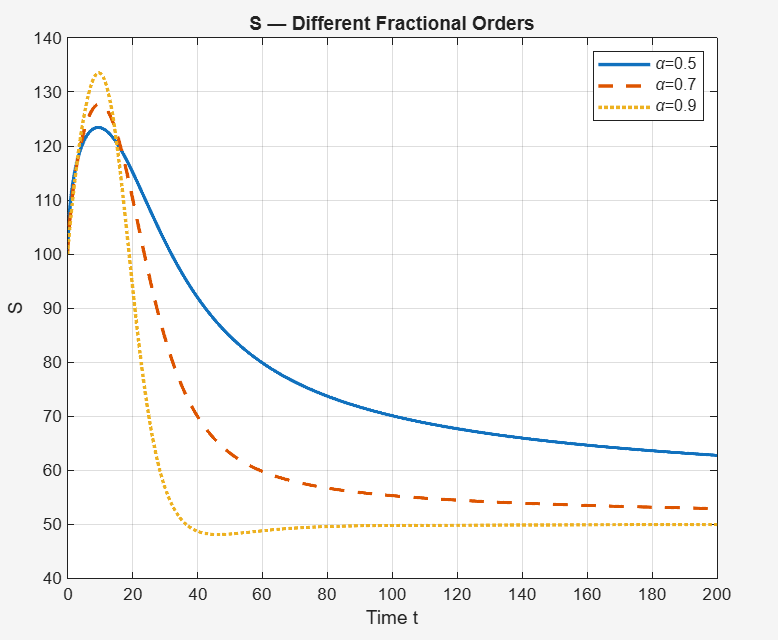
\includegraphics[width=\linewidth,keepaspectratio]{media/image1.png}
\else
  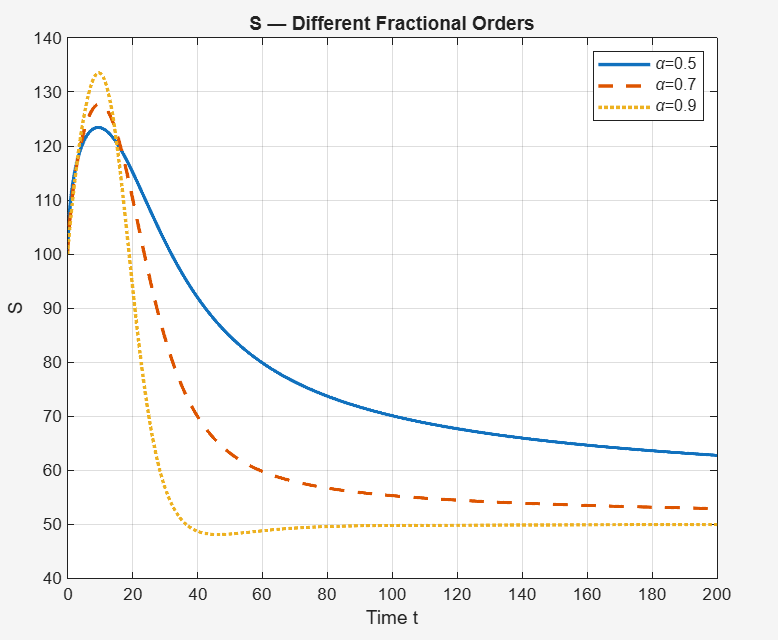
\includegraphics[width=5.9500in,height=3.6583in]{media/image1.png}
\fi
\caption{Figure 1. Temporal dynamics of the susceptible student population \(Ş(t)\)for varying fractional orders \(\vartheta\).}
\end{figure}\JLTXbelowplacement 

\JLTXaboveplacement \begin{figure}[H]
\centering
\ifdim 5.8144in>\linewidth
  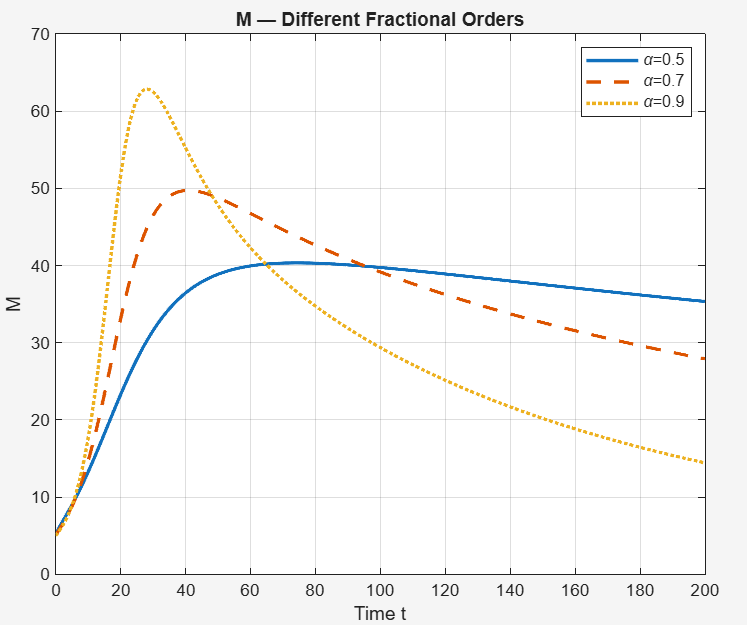
\includegraphics[width=\linewidth,keepaspectratio]{media/image2.png}
\else
  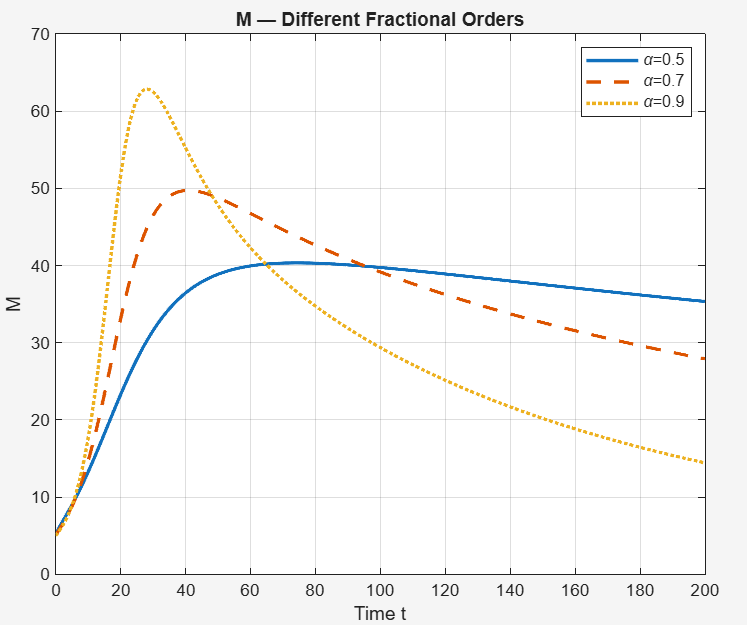
\includegraphics[width=5.8144in,height=3.8065in]{media/image2.png}
\fi
\caption{Figure 2. Dynamics of the mathphobic student compartment \(M(t)\)under different fractional orders \(\vartheta\).}
\end{figure}\JLTXbelowplacement 

\JLTXaboveplacement \begin{figure}[H]
\centering
\ifdim 5.7764in>\linewidth
  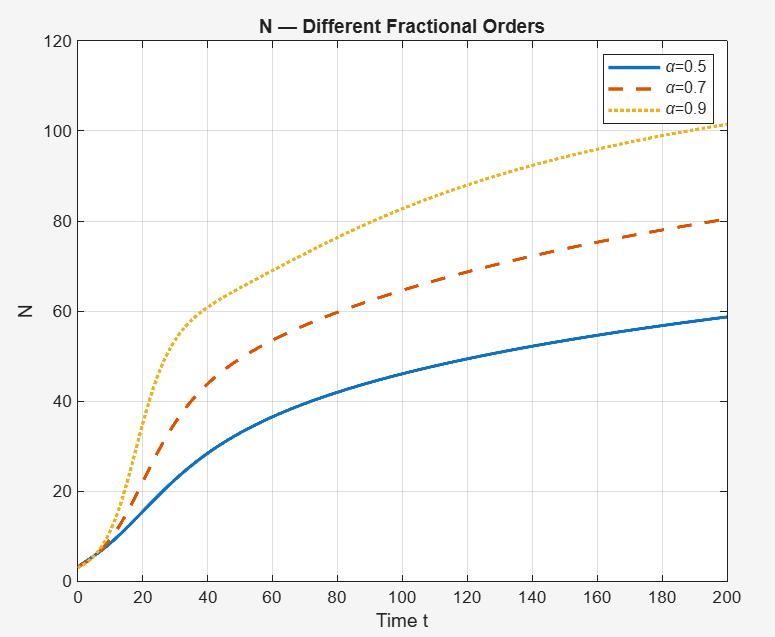
\includegraphics[width=\linewidth,keepaspectratio]{media/image3.png}
\else
  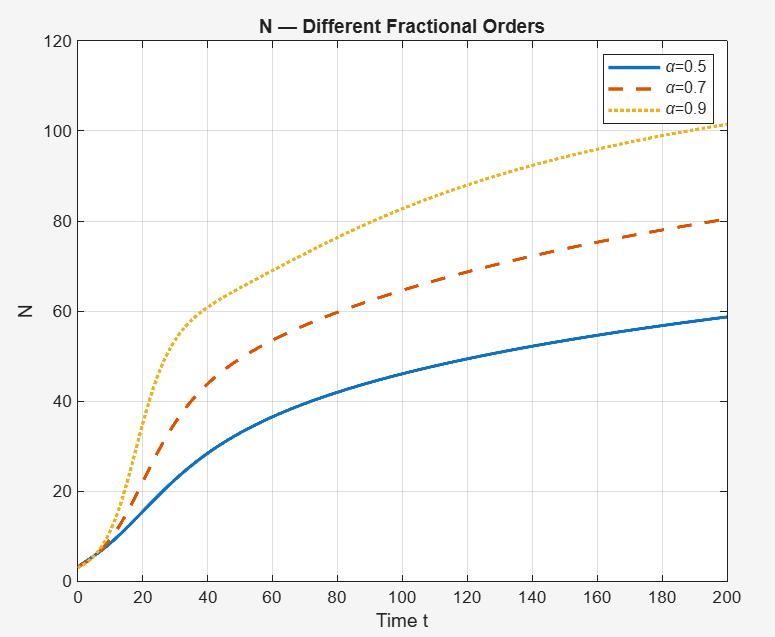
\includegraphics[width=5.7764in,height=3.3583in]{media/image3.png}
\fi
\caption{Figure 3. Variation over time of not interested students \(N(t)\)at multiple fractional orders \(\vartheta\).}
\end{figure}\JLTXbelowplacement 

\JLTXaboveplacement \begin{figure}[H]
\centering
\ifdim 5.3750in>\linewidth
  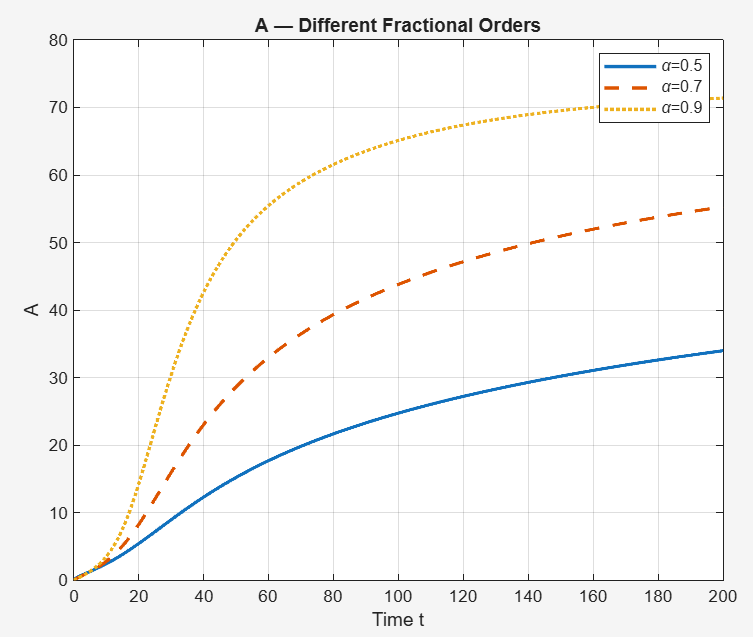
\includegraphics[width=\linewidth,keepaspectratio]{media/image4.png}
\else
  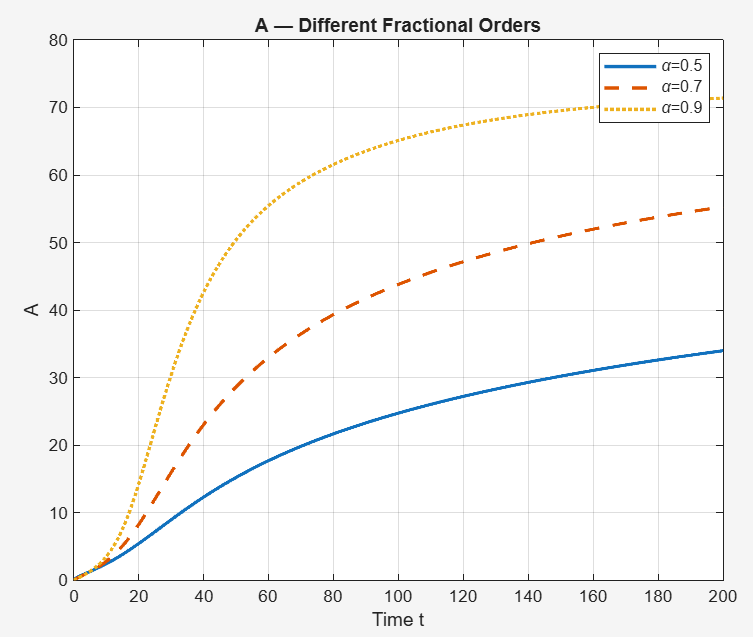
\includegraphics[width=5.3750in,height=3.2417in]{media/image4.png}
\fi
\caption{Figure 4. Trajectory of intervention-aware students \(₳(t)\)for distinct fractional orders \(\vartheta\).}
\end{figure}\JLTXbelowplacement 

\JLTXaboveplacement \begin{figure}[H]
\centering
\ifdim 5.6505in>\linewidth
  
\includegraphics[width=\linewidth,keepaspectratio]{media/image5.png}
\else
  
\includegraphics[width=5.6505in,height=3.2586in]{media/image5.png}
\fi
\caption{Figure 5. Growth and stabilization of interested students \(ƚ(t)\\)across fractional orders \(\vartheta\).}
\end{figure}\JLTXbelowplacement 

\JLTXaboveplacement \begin{figure}[H]
\centering
\ifdim 5.5005in>\linewidth
  
\includegraphics[width=\linewidth,keepaspectratio]{media/image6.png}
\else
  
\includegraphics[width=5.5005in,height=3.0669in]{media/image6.png}
\fi
\caption{Figure 6. Cumulative recovery \(Ɍ(t)\) in students as influenced by fractional order \(\vartheta\).}
\end{figure}\JLTXbelowplacement 

\par\medskip\noindent {\large\bfseries 7.Conclusion\par}\smallskip

This paper introduces a new six-compartment fuzzy fractional-order model capturing the dynamics of mathphobia in student populations, including susceptible, mathphobic, not interested, intervention-aware, interested, and recovered classes. Using Caputo-type fuzzy fractional differential equations, the model incorporates memory effects and uncertainty in transmission and recovery rates. Existence and uniqueness of solutions are established via fixed-point theory, ensuring mathematical consistency. An optimal control framework models time-dependent interventions like workshops and counseling, demonstrating through numerical simulations that combined strategies significantly reduce mathphobic and apathetic students while increasing interested and recovered individuals. This approach offers a robust quantitative foundation for designing evidence-based educational policies addressing math anxiety.

The key advantages of this work include improved behavioral realism through fuzzy fractional calculus, ability to capture long-term dependencies, and integration of adaptive control for targeted interventions. Future work could extend the model to account for social network effects, individual heterogeneity, and stochastic influences, as well as develop machine learning-based control policies for personalized anxiety management. This model lays the groundwork for more nuanced and effective approaches to mitigating mathphobia in educational environments.

Reference

\begin{enumerate}
  \item Abi, S., Zouai, O., Fessi, H., \& Ramaswamy, M. (2023). A compartmental model of TikTok addiction using SEI1I2R format: Application to social media addiction stages. Mathematical Biosciences, 350, 108900. 
  \item Alemneh, D. B., \& Alemu, A. M. (2021). Optimal control strategies for reducing social media addiction: An integrated mathematical model approach. Applied Mathematics and Computation, 410, 126476. 
  \item Ashcraft, M. H., \& Moore, A. M. (2009). Mathematics anxiety and the affective drop in performance. Journal of Psychoeducational Assessment, 27(3), 197–205. 
  \item Arshad, M. (2024). Fractional analysis of non-linear fuzzy partial differential equations and rapid-convergent analytical solutions. Nature, 628(7986), 290–299. 
  \item Ashcraft, M. H., \& Ridley, K. S. (2005). Math anxiety and its correlates. The Affective Dimensions of Math Learning, 8, 23–46.
  \item Beilock, S. L., \& Maloney, E. A. (2015). Math anxiety: A review of its cognitive consequences, and interventions. Current Directions in Psychological Science, 24(1), 52–58. 
  \item Dasumani, M., Lassong, B. S., Adu, I. K., Wireko, F. A., \& Moore, S. E. (2024). Fractional Derivative Technique for Modeling the Dynamics of Social Media Impacts. Discrete Dynamics in Nature and Society, 2024(1), 5578416.
  \item Dowker, A., Sarkar, A., \& Looi, C. Y. (2016). Mathematics anxiety: What have we learned in 60 years? Frontiers in Psychology, 7, 508. 
  \item Hembree, R. (1990). The nature, effects, and relief of mathematics anxiety. Journal for Research in Mathematics Education, 21(1), 33–46.
  \item Juhari, J., Alisah, E., Safitri, A. A., \& Sujarwo, I. (2024). Optimal Control of a Modified Mathematical Model of Social Media Addiction. InPrime: Indonesian Journal of Pure and Applied Mathematics, 6(2), 112-123
  \item Kongson, K., Gaffar, A., \& Baleanu, D. (2021). Modeling anxiety dynamics using Atangana–Baleanu–Caputo fractional derivatives. Communications in Nonlinear Science and Numerical Simulation, 96, 105715. 
  \item Liang, M., Zhang, J., \& Xu, C. (2021). Fuzzy fractional differential equations and applications to uncertain dynamic systems. Applied Mathematical Modelling, 92, 39–54. 
  \item Maayah, H., \& Arqub, O. (2023). Fractional modeling of anxiety persistence using Caputo derivatives. Fractional Calculus and Applied Analysis, 26(2), 498–514. 
  \item Momani, S., Chauhan, R. P., Kumar, S., \& Hadid, S. (2023). Analysis of social media addiction model with singular operator. Fractals, 31(10), 2340097.
  \item Mitropoulou, B., Panagopoulos, I., \& Tsanakas, J. (2022). Structural equation modelling of self-compassion's impact on math anxiety. Educational Psychology, 42(7), 908–919. 
  \item Sheinov, V. V., \& Dziavitsyn, I. A. (2021). Modeling cognitive, behavioural, and emotional interplay in addiction: A three-factor fractional approach. Chaos, Solitons \& Fractals, 144, 110695. 
  \item Van Hoa, N. (2019). Fuzzy fractional differential equations under Caputo derivative. Fuzzy Sets and Systems, 461, 98–112. 
  \item Qayyum, M., et al. (2024). Fuzzy-fractional modeling of Korteweg-de Vries equations for nonlinear waves. Applied Mathematics and Computation, 447, 127270. 
\end{enumerate}

\end{document}

















\end{document}

